\section{Background}

The types of internet connections can be usually divided in two main categories, \textbf{Generalized connectivity} and \textbf{Dedicated connectivity}.



\subsubsection{Generalized connectivity}

The most popular kind of internet connection provided by an \textit{ISP} (\textit{Internet Service Provider}), usually adopted by residential users. \\
It is based on an hierarchical structure where a set of autonomous system (\textit{AS}) communicate between each other: any two user adopting this type of connection are able to communicate using different protocols (\textit{IGP} protocol if the users are in the same AS and  \textit{EGP} otherwise).

\subsubsection{Dedicated connectivity (WAN)} \label{wans}

A specialized kind of connection, mainly used by businesses (i.e to connect the different points of sale of a large company or the different branches of a bank). \\

Organizations usually opt in into this kind of connection to ensure  higher standards in regards to different metrics (i.e lower delays, higher availability) when compared to the \textit{best-effort} approach of generalized connectivity. \\

Dedicated connectivity is still offered by internet service providers, but it is several orders of magnitude more expensive than generalized connectivity.

A network adopting this approach is called a \textit{WAN} (Wide Area Network);
a WAN is a network of LANs (Local Area Network, i.e the branches) where the distance between the LANs is usually in the tens or hundreds of kilometers range. \\
By using a \textit{border router} in each LAN, it is possibile to communicate with the other LANs in the WAN.

The LANs can be connected in different ways:
 

\begin{enumerate}
	\item \textit{Dedicated physical WAN} : the business buys the full physical infrastructure that the networks is built on (the cables, the switches etc.). \\ While the company is the owner of the whole WAN, the cost is extremely high and network management (e.g enforcing security) is the the company's responsibility.
	
	\item \textit{Leased Lines} : the business relies on an ISP to establish private circuits between the branches. (e.g branch 1 must be connected to branch 2, which must be connected to branches 3 and 4) \\
	The private circuit may be created by assigning  a dedicated wavelength to a particular customer. \\
	This solution offers only partial control, but is cheaper and offsets some of the network's management issues to the ISP.
	
	\item \textit{MPLS networks}: The business still relies on an ISP to provide connectivity, but unlike leased lines there are no established circuits between the branches.  Instead, a mesh connectivity is provided , with a certain QoS guarantee. \\
	For each branch a \textit{customer edge router} is installed, allowing the branch to access the MPLS network via a \textit{provider edge router}. \\
	The \textit{provider edge router} (PE) is in between the MPLS network and the companies, one PE may manage connections for multiple customers.
	
	\item \textit{SD-WAN}: this kind of WANs will be discussed in detail in the next section.
	
	
	
\end{enumerate}


\begin{figure}[h!]
	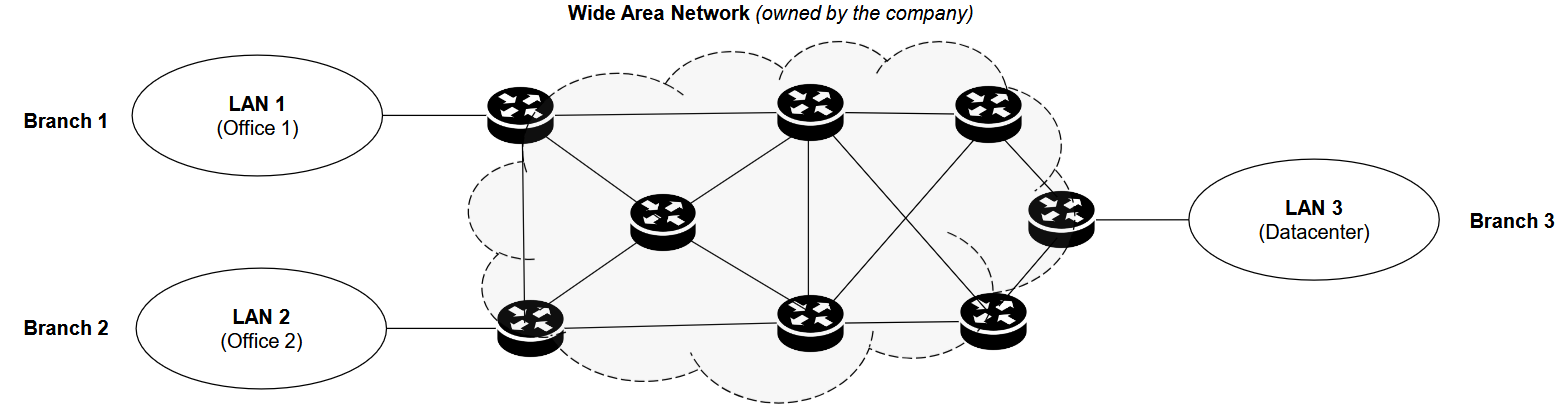
\includegraphics[width=\textwidth]{private_wan}
	\caption{A sample network adopting a dedicated wan}	
	\centering
\end{figure}

\begin{figure}[h!]
	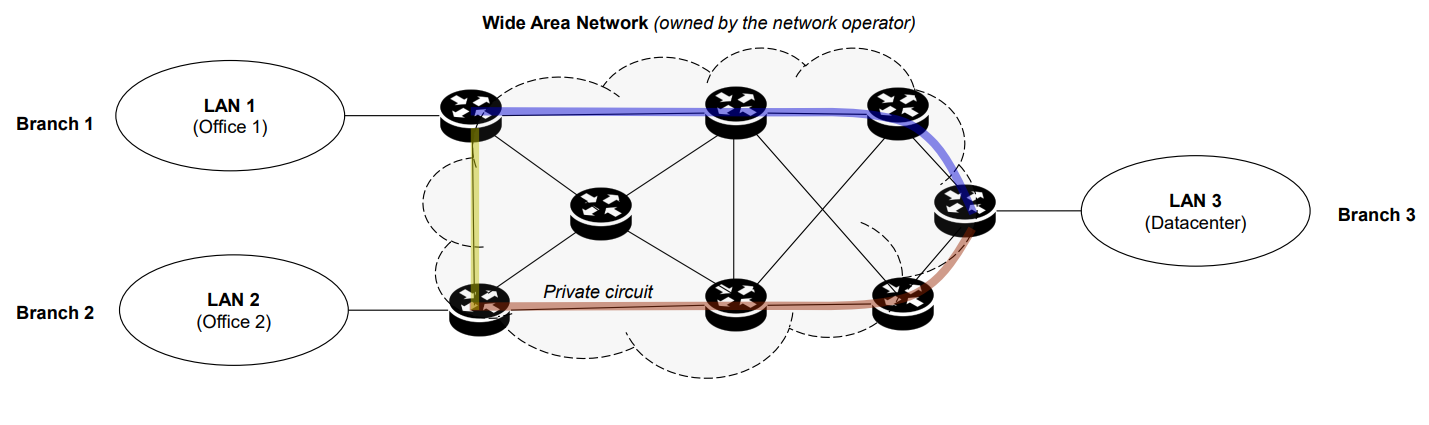
\includegraphics[width=\textwidth]{leased_lines}
	\caption{A sample network using leased lines. The different colors show the different link between the branches}	
	\centering
\end{figure}

\begin{figure}[h!]
	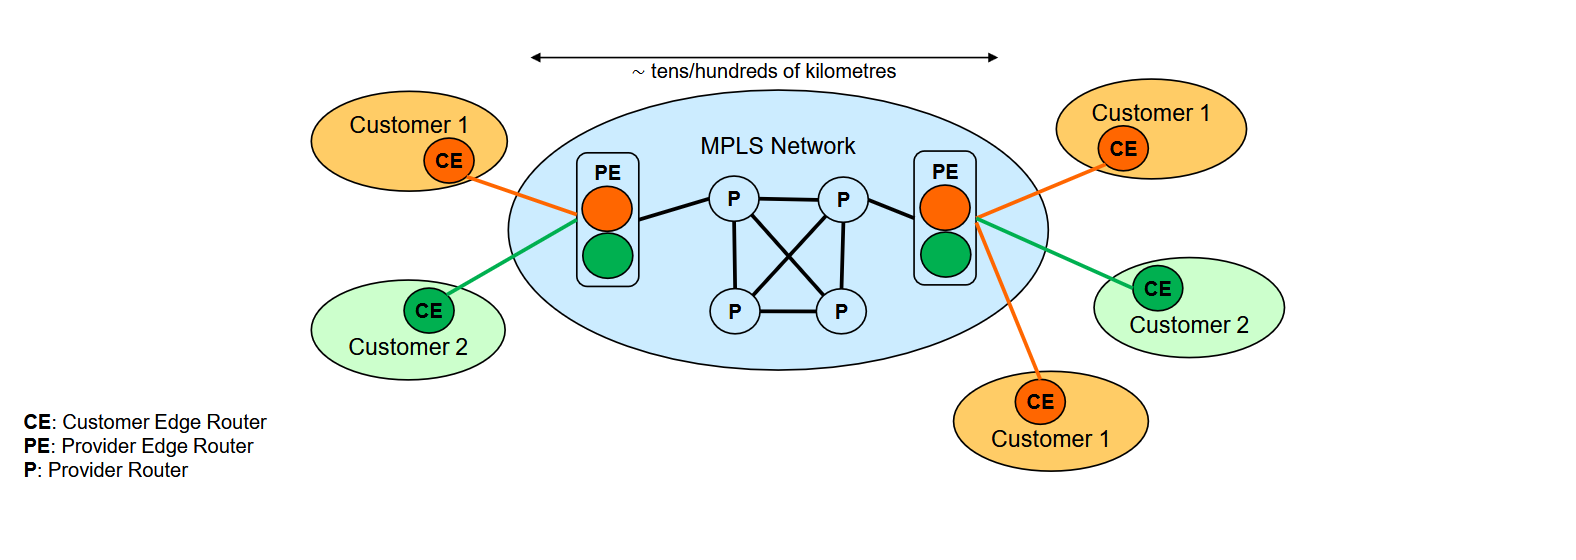
\includegraphics[width=\textwidth]{mpls}
	\caption{A sample network using MPLS}	
	\centering
\end{figure}

\vspace{0.2cm}

\section{Software defined networking and SD-WAN}

\subsection{Networking devices}
A typical network device (e.g routers, firewalls...) is usually composed by two logical components:
\begin{enumerate}
	\item A data plane 
	\item A control plane
\end{enumerate}

The data plane is used to handle individual data packets locally.
For example the data plane in a router is used to determine to which interface a packet should be forwarded to.
The data plane usually applies a large amount of small, fast operations. \\
The control plane is used to handle control messages from other devices in the network, and allows the network device to work from a network wide perspective. \\
The messages from other devices may be  used to configure policies which are then applied by the data plane (e.g the control plane receives a policy that determines which packets should be filtered, while the data place does the actual filtering). \\
Compared to the data plane, the control plane is used for more complex operations that usually require coordination along network devices.

\vspace*{0.2cm}
\begin{figure}[h!]
	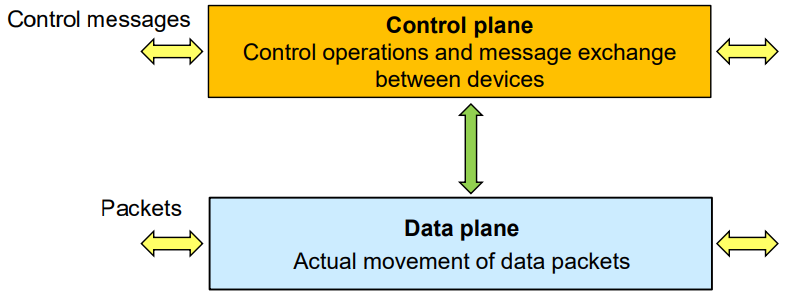
\includegraphics[width=0.75\textwidth]{control_and_data_plane}	
	\centering
\end{figure}



\subsection{Definition}
The idea behind software defined networking (SDN) is to de-couple the control plane from the data plane, not only on a logical level but also physically \cite{6834762} .

The control plane is no longer part of the network devices and is instead moved to a  centralized software component called a \textit{controller}.

The basic architecture of a SDN is composed by the controller and by a series of network devices which in this context are called \textit{switches}.


A SDN controller

\begin{enumerate}
	\item Is able to communicate with the switches
	\item Can be programmed: it is now possible to write software that defines how the whole network behaves. \\
	The switches keep executing their data plane locally, according to the policies received by the controller.
	\item Is able to acquire information about the network it is managing, e.g it can discover the topology of the network to know where the switches are places and how they are connected.
\end{enumerate}

The goal of the controller is to communicate with all the switches to inject into them the desired network behavior

The controller is logically placed between the network infrastructure and the application layer.

Using a series of high level programmable interfaces  (also called \textit{APIs} A\textit{pplication} \textit{P}rogrammable \textit{I}interfaces) the controller is able to communicate with its neighboring layers.


Using the APIs connected with to the application layer (the \textit{northbound}) interfaces various network devices can be implemented, e.g a network balancer, a firewall.

The communication between the controller and the switches is made possibile by a series of \textit{southbound} interfaces.

Using these interfaces the controller can effectively apply the policies to the network, e.g it can send traffic rules to the switches connected to the controller.

Inside each switch there is a set of \textit{generic tables} (also called \textit{flow tables}) that are used to store the configuration sent by the southbound interfaces.

The southbound interfaces can also be used in "reverse": the switches are able to communicate with the controller using a series of predefined messages.

\begin{figure}[h!]
	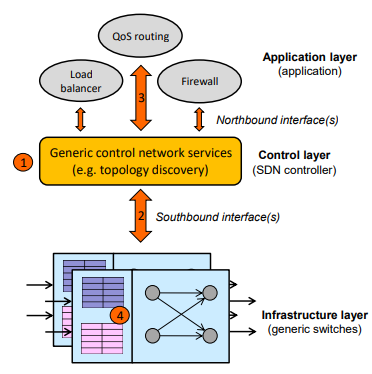
\includegraphics[width=\textwidth]{sdn}
	\caption{The main components of SDN}	
	\centering
\end{figure}



\subsection{Openflow}
Despite being relatively new \cite{openflow} , software defined networking became a popular approach for organizing new networks (e.g in 5G networks).
Compared to other widespread network technologies such as the TCP/IP stack, software defined networking is a relatively new approach: the first paper defining protocol for SDN (the \textit{Openflow Protocol}) was published in 2008.

The OpenFlow protocol defines a sets of API for remote communication with network plane devices, i.e. a southbound interface.


SDN switches inside the context of OpenFlow are also called \textit{generic} switches;
This is to avoid confusion with the usual meaning of the term switch, which usually refers to a device used to manage level 2 functionalities (i.e. the data link level, used to handle the physical addressing with MAC addresses). 
Openflow switches are able to interact up to the fourth layer (i.e. the transport layer, which may include protocols such as TCP or UDP).

A large portion of an OpenFlow Switch is composed by functionalities related to the data plane, the only portion dedicated to the control plane is delegated to the \textit{control channel}.

The control channel includes one or more OpenFlow channel that allows the switches to communicate with one or more controllers (multiple controllers may be used to avoid a single point of failure in the infrastructure).
 
OpenFlow switches include three kind of tables, used for handling data plane functionalities:

\begin{itemize}
	\item \textit{Flow tables}: the most important kind of table, they can be chained in a pipeline. \\
	They contain the rules that are applied to the incoming and outgoing traffic.
	\item \textit{Group tables}: Users of a SDN can be assigned to different group; group tables allow traffic to be sent in multicast to users of a specific group (e.g. group tables can be used to send outgoing traffic to multiple ports if necessary)
	\item \textit{Meter table}: table used to collects statistic about the current network. \\
	The gathered data can then be used to handle QoS (e.g rate limiting for traffic directed to a specific port)
\end{itemize}

\subsubsection{Configuring the tables}
To work properly, the flow tables inside the switches have to be configured by the controllers in the network.
The solution is usually an hybrid of two types of configuration:
\begin{enumerate}
	\item \textit{Proactive configuration}: When the switch is first inserted into the network, the controller proactively fills the tables. \\
	The entries in the tables are static and do not change across the lifespan of the switch in the network. \\
	This kind of approach is obviously unfit for rapid changing scenarios such as those encountered in managing networks.
	\item \textit{Reactive configuration}: Initially there no entries in the flow tables; the tables are fully configured at runtime according to the network state. \\
	If a switch does not known where a package should be send to, it forwards the packet to the controller. \\
	The controller is aware of the full topology of the network, and is then able to edit the received package to include the routing information, before sending the package back to the switch..\\
	This leads to increased round trip time for the first packets sent across the network. \\
	However, communication between the switches and controller usually represent a bottleneck for the network's performance; a large amount of packets sent to and from the controller may cause congestion in the network and limit the available bandwidth.
\end{enumerate} 



Usually the preferred solution is based on an hybrid approach. \\
A starting set of rules is used at the start up of the network, to cover the expected data flows in the network. \\
For any unknown data flow that may arise during the lifespan of the network new routing rules will be issued by the controller.

\begin{figure}[h!]
	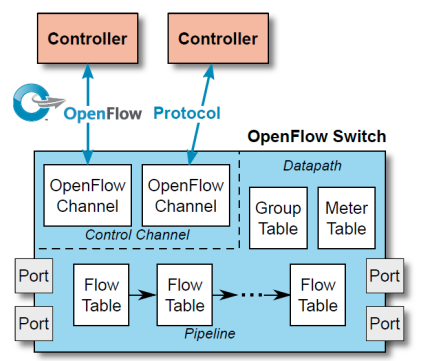
\includegraphics[width=\textwidth]{openflow}
	\centering
\end{figure}


\subsection{SD-WAN}

\subsubsection{SD-WAN}
The principles of software defined networking can be applied when building a WAN;
while SD-WAN were introduced recently (in 2014) their popularity increased due to the possible decrease in costs when compared to traditional WAN solutions.

SD-WAN works by stipulating multiple contracts of generalized internet connections (e.g 4G, POM, fiber) and then combining the different networks to guarantee a certain quality of service level.

Like the MPLS approach, a CPE (\textit{Customer} \textit{Premises} \textit{Equipment}) is installed in each branch of the business.

The CPEs is connected to the branch's LAN and to multiple generalized connectivity networks.

The traffic generated by the LAN may then travel in different networks, potentially even from different ISPs.

An SDN controller, in this specific context called an \textit{SD-WAN Controller} is responsible to communicate to each CPE how the outgoing traffic should be managed (e.g two branches may be connected using a fiber cable, if the cable connection fails the controller will instruct the branches to communicate using a 4G network ).

MPLS may still be used in a SD-WAN context, a company could decide to use other (usually cheaper) kind of connections for most use cases and reserve a MPLS connection only exceptionally.

\pagebreak

\begin{figure}[t]
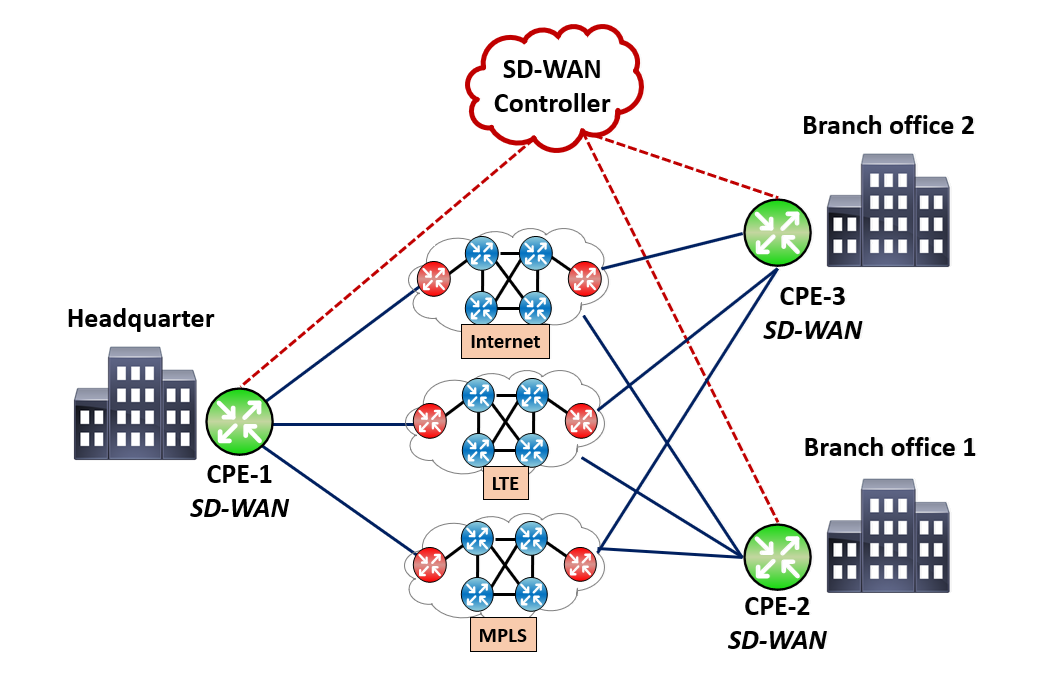
\includegraphics[width=\textwidth]{sd_wan}
\caption{A sample network of three branches adopting SD-WAN}

\centering
\end{figure}


\subsubsection{Load balancing and SLA in SD-WANs}

As we previously discussed, in SD-WANs a controller's task is to instruct CPEs on how they should distribute outgoing traffic among the available links. \\

The traffic handled in a SD-WAN context is often heterogeneous and generated by different applications (i.e VoIP, emails, video streaming \dots).

Different applications have usually varying requirements in regards to the acceptable delay and the packet loss that can happen during the transmission of data.

Two important terms have to be introduced to describe the needs of each network application:
\begin{enumerate}
	\item \textit{QoS (Quality of Service)}: a quality indicator used to measure the service level of a given network communication.  It is defined with a series of guarantees that must be respected during a network communication. \\
	In this paper QoS will always be defined in absolute terms (e.g. end to end latency is less than 5 milliseconds,  2\% of packets have been dropped), however it can also be defined in relative tems (i.e how a given traffic flow is   treated with respect to the others)
	\item \textit{SLA (Service Level Agreement)}: the SLA specifies the QoS that has to be guaranteed for a given application. It provides a series of bound on various measurable parameters (i.e the latency \textit{must} be less than 5 milliseconds)
\end{enumerate}

